\chapter{Literature Review}
\label{chap:LitReview}
%This section will first cover previous research done in the fields of ECG, SpO2/PPG, and acceleration sensors. Then a discussion of how to derive synthetic sensor measurements based on acquired ECG, SpO2/PPG, and acceleration measurements. I will focus on literature with methods of deriving heart rate, blood pressure without a cuff, and deriving respiration rate without a chest strap. Next, I will present methods for removing noise from the ECG and PPG sensors based on accelerometer data. Finally, the pertinent literature in the medical domain will be review, paying specific attention to the fields of patient education and self-care as well as the psychosocial instruments to be used, the MLHF, DASI, and HFSA.

\section{Prior Research}
\label{sec:priorResearch}
There are numerous related research areas affecting the proposed work, including existing standards (e.g. sensors, wireless, heath, and health ontologies.), physical and synthetic sensors, and data fusion/classifications. Each topic is briefly examined, in the following sections, as related to the dissertation's research effort.

\subsection{Existing Standards}
\label{sebsec:ExistingStandards}
In order to promote adoption of the WHIPPED system, sensor standards, wireless-standards, healthcare-standards, and health ontology-standards are examined. 
Sensor standards are examined that may affect the design of the sensor patch. 
Wireless standards are examined to determine the best way to transmit biometric data to the smartphone. 
Finally, health standards, and health ontology-standards are examined to find trends in the storage, transmission, and classification of health information and disease classification.

\subsubsection{Sensor Standards}
\label{subsec:SensorStandars}
Data from the sensor suite must be interpreted by the control microprocessor and transmitted to the patient's phone consistently. Different protocols for sensor data interpretation and transmission already exist.  The Open Geospatial Consortium Inc. (OGC) is developing an initiative called Sensor Web Enablement (SWE) \cite{Botts2007a}. SWE is a collection of open standards designed to make any type of sensor plug and play. SWE is made up of several standards such as Sensor modeling language (SensorML) \cite{Botts2007}, and Transducer modeling language (TransducerML), among others. SensorML represents a standard way for providing specifications for a sensor device. Only a subset of the large amount of metadata provided by SensorML is needed. TransducerML defines a self-describing protocol based on XML to support data transmission between any type of sensor and data sink \cite{Fortier2009}.

These standards propose a heavyweight approach to sensor identification and interoperability. SWE allows any sensor to be seamlessly integrated into a system. The research approach is to use a fixed set of sensors. The high overhead of SWE makes it unsuitable for the dissertation's research. However, meta-data concerning the transducers is still needed. A more lightweight approach using IEEE standard 1451.4, Transducer Electronic Datasheets (TEDS) is proposed. Most smart transducer's TEDS use a memory device attached to the transducer, which describes the transducer's identification, calibration, correction data, measurement range, manufacturer related information, and so on. TEDS allow us to be relatively free with hardware choices by allowing the software to read the required information from the sensor patch. Many versions of the sensor patch hardware can integrate seamlessly with one software platform by providing TEDS. \cite{IEEE1451_4}


\subsubsection{Wireless Standards}
\label{subsubsec:WirelessStandards}

\begin{figure}
	\begin{center}
		\label{fig:WirelessComparison}
\begin{tabularx}{1\textwidth}{>{\bfseries}p{.23\textwidth}||p{.25\textwidth}|p{.15\textwidth}|p{.25\textwidth}}
\hline Standard 			& Wi-Fi & Bluetooth & ZigBee  \\\hline
\hline IEEE Spec. 			& 802.11 a/b/g & 802.15.1  & 802.15.4  \\
\hline Frequency Band 		& 2.4 GHz; 5 GHz & 2.4 GHz & 868/915 MHz\par2.4 GHz  \\
\hline Max \par Signal Rate 		& 54 Mb/s & 1 Mb/s & 250 Kb/s \\
\hline Nominal Range 		& 100 m & 10 m & 10 – 100 m  \\
\hline Nominal TX Power 	& 15 – 20 dBm & 0 – 10 dBm & (-25) – 0 dBm \\
\hline Number Of RF Channels & 14 (2.4 GHz) & 79  &  1/10; 16 \\
\hline Channel \par Bandwidth 	& 22 MHz & 1 MHz  & 0.3/0.6 MHz; 2 MHz \\
\hline Coexistence Mechanism& Dynamic freq. \par selection, transmit power control (802.11h) & Adaptive freq.\par hopping & Dynamic freq. \par selection  \\
\hline Maxi. nodes & 2007 & 8 & 65000 \\
\hline Encryption 			& RC4 stream cipher (WEP),\par AES block cipher & E0 stream cipher & AES block cipher \par(CTR,\par counter mode) \\
\hline Authentication 		& WPA2 (802.11i) & Shared secret & CBC-MAC \par(ext. of CCM) \\
\hline Data Protection 		& 32-bit CRC & 16-bit CRC &  16-bit CRC \\
\hline 
\end{tabularx} 
		\caption{Comparison of wireless technologies}
	\end{center}
\end{figure}


Collecting, and interpreting, sensor data is only part of the problem statement. A useful device must transmit data for further processing. Several standards and architectures for data transmission were considered. A wired connection to a smartphone was quickly discarded. While it would offer a simple and fast communication to a comparatively more powerful device, it is obtrusive and introduces a hazard to movement that could exert a strain on both devices if the cable became caught on another object. Therefore, several methods of wirelessly transmitting collected data were researched. Many technologies make use of the ISM 2.4 GHz band; Bluetooth, ZigBee and Wi-Fi fall into this category and were examined.  Shannon compares Wi-Fi, Bluetooth, and ZigBee in his master's thesis \cite{Shannon2012}. Wi-Fi offers the highest throughput and range but at the cost of extreme power usage. Bluetooth has the next highest throughput at much more acceptable power consumption. ZigBee offers the most customization and is capable of supporting up to 65000 devices in a single network, however is lacks smartphone communication support.

While ZigBee meets the minimum bandwidth requirement, as shown in \cref{fig:WirelessComparison}, and uses less power, Shannon concludes the lack of smart phone hardware support makes Bluetooth a better option presently. If phones begin supporting the ZigBee protocol a switch could be made, in the future.  ZigBee could be a viable protocol in the future as shown by Peligris; who examines the IEEE802.15.4\cite{IEEE802.15.42011}, the protocol underlying ZigBee \cite{Pelegris2011}.

Bluetooth is a wireless technology standard for exchanging data over limited distances. It supports many profiles including: hands free profile, a stereo audio profile, and serial port profile. Noueihed et al. compare two profiles for the transmittance of biometric data. The Serial Port Profile (SPP) is compared to the recently released Health Device Profile (HDP). The results of the analysis indicate HDP offers better reliability in some cases of interference, episodic transmission interference, and equal reliability in others, voice type interference \cite{Noueihed2010}. However, hardware support for HDP is currently scarce while support for SPP is nearly universal in Bluetooth modules. Bluetooth SPP is used for the remainder of the dissertation. However, the application shall be designed modularly with the transition to HDP planed when better hardware support is available.

A primary driver in the component analysis is the Space, Weight, and Power and Cost (SWaP-C) of the selected protocols and hardware support. Wi-Fi offers an unacceptably high power requirement. ZigBee has no hardware support for the WHIPPED platform. Bluetooth SPP provides an acceptable power requirement and suitable data transmission rate.

\subsubsection{Health Standards}
\label{subsubsec:HealthStandards}
Usually if a patient receives home care services, they are seen within one week and the interval is determined by the nurse responsible for the patient. Home care patients are typically followed for at least 90 days depending on how sick they are. A nurse is sent to the patient's home to assess the patient's status. Typically, between discharge and the first in-home visit, the patient does not interact with health care providers unless they seek assistance from their local primary health care provider. Gustafsson shows 25\%-50\% of hospitalized patients will be readmitted within six months of their initial hospitalization \cite{Gustafsson2004}. Further, Lee et. al would seem to indicate 25\%-30\% of CHF patients will die or have another hospitalization within the first 30 to 60 days \cite{Lee2011}. Lee and Gustafsson's findings underscore the need for better communication during those crucial first days and weeks after a patient leaves the hospital.

Agreeing on a common frame of reference is an essential part of the communication between clinician and patient.  Frequently elderly patients ignore symptoms of CHF because they attribute the pain(s) to “getting older” and not as a sign of a deteriorating condition. Several psychosocial and symptom tools have been produced enabling patient assessment by asking simple questions ranked on a likert -1 to five, scale. The Duke Activity Status Index (DASI) is a 12-item questionnaire with a score which can be translated into an estimated peak oxygen intake in mL/min \cite{Hlatky1989}. More commonly, the DASI is an indicator of energy levels used and is a general measure of activity.  Often patients with heart failure will decrease activities in the presence of worsening symptoms. Therefore, looking at the pattern of activity levels and symptoms provides a fuller picture of the patient's cardiac status. The Minnesota Living with Heart Failure Questionnaire (MLHFQ) is a 21-item questionnaire also using a likert scale \cite{Jurgens2009}. The MLHF-instrument measures patients' perceived QOL, and how much symptoms interfere with QOL. Repeated responses the MLHFQ strongly correlate to the New York Heart Association's (NYHA) classifications. The Heart Failure Somatic Awareness Scale is a 12 item likert scale developed to measure somatic awareness and perceived severity of symptoms specific to heart failure \cite{Jurgens2006}. All of these instruments can be used to augment and correlate with the biometric readings collected by the sensor device. Additionally, repeatedly administering these assessments can track changes in the self-perceived status of a patient. Establishing how patients perceive their own wellness is an important factor in treatment. Finally, educating a patient about the differences between their perceived status and actual status can be useful in a patient's self-care and rehabilitation.

The dissertation uses primarily the HFSA, DASI, and MLHF as instruments. The focus of the work is not development or validation of these instruments; that has been done in previous studies over an extended period, with thousands of patients.

\paragraph{Electronic Health Records (EHR)}
\label{par:ElectronicHealthRecords}
Some of the most important medical standards are still being written. An electronic health record (EHR) is a way of representing, and storing digitally, every medical piece of information about a patient. Data can be anything from patient demographics to an MRI scan or ECG data, temperature, weight, etc. The American Medical Informatics Association (AMIA) is working on developing a standard set of components for an EHR. Another, standard under development involves how information of various formats should be transmitted across different EHR systems. Both ANSI-X12 and HL7 are developing standards for electronic data interchange. When completed, an EHR will be a longitudinal record of every interaction a patient has had. The use of a subset of the EHR standard, mostly concerning the demographics of a patient and any history of heart disease and co-morbid illnesses will be sufficient for current research.

\paragraph{Health Ontology}
\label{par:HealthOntology}
When a clinician is diagnosing a patient, they often refer to clinical practice guidelines (CPGs). CPG are documents written for clinicians that provide evidence-based best practices. Given a set of symptoms, and patient demographics, a course of care can be prescribed to achieve a desired outcome. A full medical ontology would provide an exhaustive list of the domain of symptoms correlated with all possible demographic data and provide options for improving patient's conditions. A minimal database would be more than is necessary for the dissertation.

Jones et al. show a method of converting a CPG to an XML based representation aimed at generating tailored educational material for clinicians \cite{Jones2005}. A large portion of development time was spent generating the educational material and converting the CPGs to a computer format.  Many other approaches to representing CPGs electronically have been proposed, including EON, GEODE-CM, N-CODES\cite{Peleg2003} and the Asgaard project\cite{Shahar1998}. Shah proposes one additional method, Proteus\cite{Shah2001}. Proteus method focuses, not on the initial creation of the ontology but, on the maintenance, modification, and updating of the ontology.  By providing the ability to easily edit a large database of knowledge Shah suggests using a system such as PROTEUS will promote faster adoption of electronic health ontologies [11].

We are using a partial health ontology focused on chronic cardiac patients in the research. The ontology supports definitions of symptom and symptom-severity, classifications of patients into the New York Heart Association's classes, appropriate interventions, and co-morbidity diseases. The intent is to aid in fast classification of patients and to detect patients in outliers.


\begin{figure}
	\begin{center}
		
		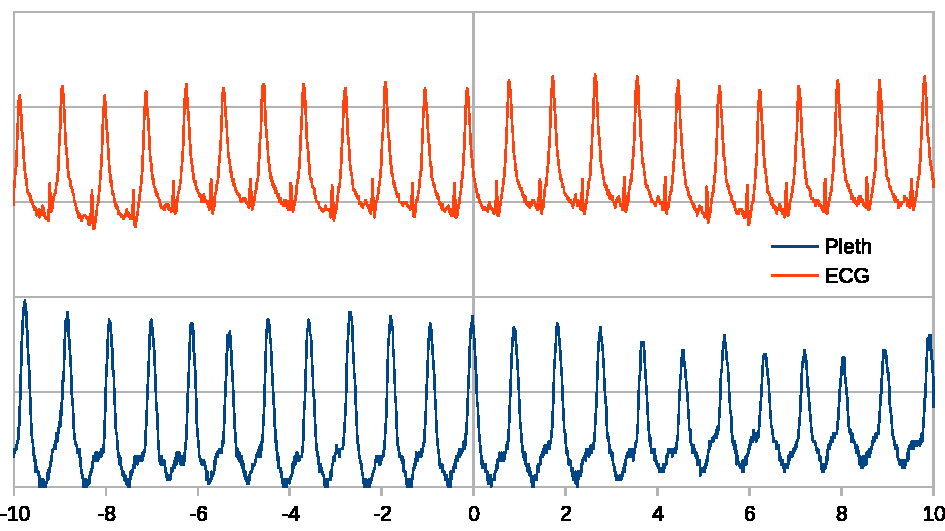
\includegraphics[scale=1,width=0.9\textwidth]{Images/20second.pdf} 
		\caption{Twenty Second Captured Trace of WHIPPED Version2 ECG and SpO2 waveforms}
		\label{fig:20SecondEcg}
	\end{center}
\end{figure}


\subsection{Sensors}
\label{subsec:Sensors}
When examining relevant research in sensors only sensor technology related to specific biometric measurements requirements is considered. The focus of the dissertation's efforts is not in analog transducer front-end research, but in smart sensor research design, development, and implementation to meet requirements of a SWaP-C smart patch. If the traditional hospital sensor suite from a trauma ward was used, then number of discrete measurements and required footprint of the hardware would far exceed the SWaP-C goals upon which the research was initiated.

Some metrics, such as: ECG, O2-Saturation (\spo2), Blood pressure(BP), pulse rate, respiratory rate, blood flow rates, and temperature are considered when evaluating the health of a patient's heart. The patient's ECG reading and their O2 Saturation are of key importance. A sample recording of an ECG and \spo2 waveforms is shown in \ref{fig:20SecondEcg}. Remaining required heart metrics can be derived from the ECG and \spo2, as will be discussed in the synthetic sensor section. Space, weight and power with respect to cost (SWaP-C) can be minimized by focusing on minimizing the number of transducers. Having fewer sensors meshes with the project research goals of an easy to use, and cost effective, device that requires little or no medical knowledge to use.

\subsubsection{Electrocardiogram (ECG)}
\label{subsubsec:Electrocardiogram}
Electrocardiography (ECG) is used to measure the electrical activity of the heart. Clinicians are able to detect abnormalities such as tachycardia, bradycardia, and atrial and ventricular fibrillation among others by monitoring a patient's ECG . Traditional techniques measure the potential of between 2-12 electrodes, or leads affixed to a patient. These signals have very small potentials between them and require an analog front end to produce readings, which can be easily digitized. Numerous techniques for acquiring an ECG signal have been presented in the literature \cite{Kim2011,Yan2011,Faggion2011,Secerbegovic2011}.  When considering a compact sensor device, the number of leads is a prime concern. Therefore, many two and three lead device designs were considered. Two leads are the minimum required to detect potential voltage across the heart. The third lead is used to inject a small current back into the patient as active noise cancellation. The three-lead technique is used in current reference designs \cite{TI2006} . Another novel approach detected a patient's ECG from a distance using two aluminum discs \cite{Belgacem2011}. However, detecting an ECG, from a distance, applies only to immobile patients. Variations in the distance to the patient yielded unpredictable results, which precludes it from use in ambulatory patients and in mobile home-care patients. 

Capturing an ECG signal is the first step in assessing patient health. A healthy ECG signal will demonstrate several peaks and valleys for each heartbeat. Each of these Principally Important Points (PIPs) represents an action happening in the heart. The PIPs are labeled PQRST. The P wave represents depolarization of the upper part of the heart, called the atria. A normal maximum P wave duration is ~100 mS. The time between the beginning of the P wave and the peak of the R wave represents the time required for an electrical impulse to depolarize the atria and reach the electrical conduction system of the lower part of the heart, called the ventricle. The normal P-R interval in a healthy adult is 120 mS to 200 mS. Together the QRS PIPs are called the "QRS complex" and they represent ventricular depolarization. Finally, the T wave represents ventricular re-polarization. The time between the Q and T waves, the Q-T interval, represents the time when the heart is unable to be depolarized \cite{Khorovets2000}. Deviations from these accepted norms represent a problem with the normal sinus rhythm. Additional processing of the raw ECG waveform can identify these abnormalities.

The dissertation's research, does not seek to revolutionize the acquisition of the ECG waveform. Rather, it seeks a preexisting robust method, using a minimum of leads and components. Based on the results indicated in the literature surveyed, the dissertation will more closely follow a two-lead approach. The analog front-end design, uses minimal gain and filtering components opting instead to use a high accuracy Analog to Digital Converter (ADC) and minimal gain. The proposed approach simplifies the system design and allows for sufficient resolution to detect small artifacts in the signal and preserve the baseline drift for the synthetic sensor measurements. A more detailed approach to ECG capture can be found in "\cref{sec:ResearchDoneToDate}"



\subsubsection[Photoplethysmograph(PPG)]{Photoplethysmograph (PPG)/ Oxygen Saturation (\spo2)}
\label{subsubsec:Photoplethysmograph}
The second transducer researched is used in measuring patient oxygen saturation (\spo2). The respiratory system of a human body takes in oxygen from the air into the lungs where oxygen is extracted. The absorbed oxygen is transferred to the blood cells for distribution to the rest of the body. Depending on the health of a patient, the level of oxygen in the blood at any moment can vary. \spo2 is a percentage of oxygenated blood cells versus non-oxygenated blood cells. The \spo2 metric does not identify the number of oxygenated cells; only the ratio of oxygen carrying cells (HbO$_2$) to the non-oxygen carrying cells (Hb). The absorption spectra of the two types of cells are different as shown in \cref{fig:Hemoglobin}\cite{Prahl1998} can be used to identify the ratio. Two waveforms are acquired by exposing the body to two different wavelengths, 660 nm (Red) and 940 nm (Infrared), and measuring either the transmittance or reflectance of the patient. These signals can then be used for additional processing. Pulse rate, \spo2, and respiration rate all require the PPG waveform \cite{Scully2012,Kraitl2011}.  Some research has suggested it is possible to measure blood perfusion based on a PPG however, this approach has only been tested on babies \cite{Noor2011}.


\begin{figure}
	\begin{center}
		\label{fig:Hemoglobin}
		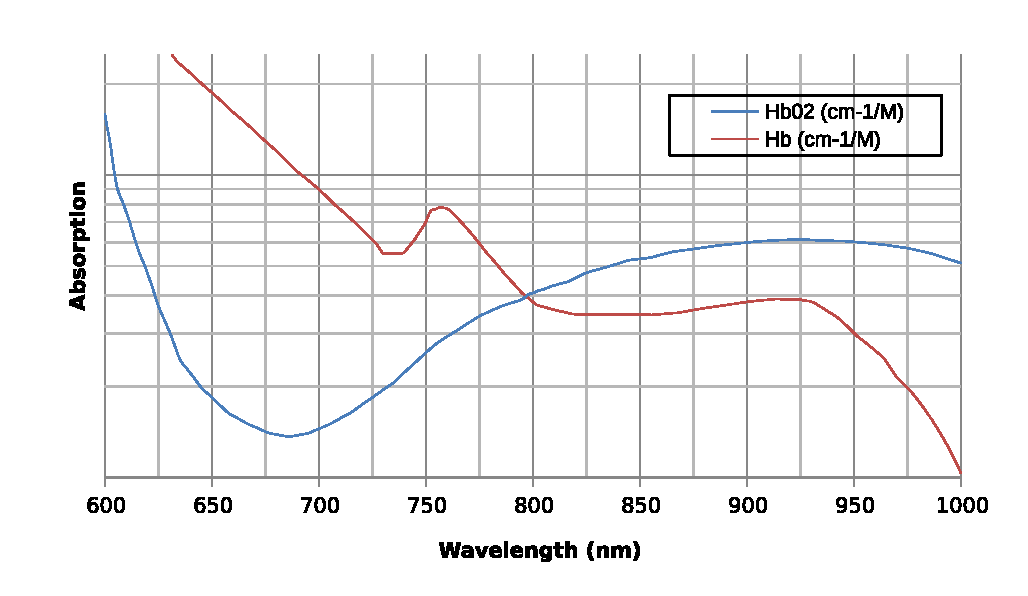
\includegraphics[scale=1,width=0.9\textwidth]{Images/hemoglobin.pdf} 
		\caption{Absorption Spectra of HbO2 (dashed) vs. Hb (Solid) }
	\end{center}
\end{figure}

For a single transmittance measurement the resulting value depends on several factors. First, the reading will fluctuate based on the amount of tissue the light must pass through. However, the amount, and density, of tissue varies with time. Further accentuating the problem, the most important component of the signal accounts for only 2\% of the magnitude of the signal. Front end processing usually removes the non-pulsatile part of the waveform leaving only the pulsating part, called a plethysmograph. The resulting graph shows only the time varying signal, allowing for larger magnification of features \cite{Jawahar2009}.

One goal of the dissertation is to have an integrated smart patch located in one area of the body. The optimal location for measuring ECG is over the heart, while for O$_2$ Saturation the optimum location for a transmitve sensor is a finger or earlobe. Reflectance sensors do not have such limitations. Part of the research is to determine alternate sites for PPG measurement with a reflective sensor near the heart that provides adequate resolution.

\subsection{Accelerometers}
\label{subsec:Accelerometers}
An accelerometer is a device capable of measuring changes in acceleration, in three dimensions. Recently, cost and size of these devices have decreased a result of Micro Electro-Mechanical Systems (MEMs);  Previous group research has shown it is possible to use acceleration data to augment the classifier algorithms to adjust for changes in motion \cite{Shannon2012}.  Outside research has also presented methods for on body device localization \cite{Vahdatpour2011}. 

Part of the proposed research is to integrate acceleration data into the calculations for heath metrics. Combating noise and motion artifacts is a prime concern since, in the research, low-noise waveforms for ECG and PPG are required to provide meaningful data.

While some methods focus on noise removal through activity-unaware means such as wavelet transforms \cite{Liu2011} the dissertation proposes using the accelerometer data in two ways. First, minimally, the acceleration data can provide a confidence level to the acquired waveforms. One option is binary movement analysis, where the result is either “moving” or “not moving”, the classifier can choose to accept or discard the acquired readings. Movement can be correlated with changes in the ECG and PPG waveforms for a fine tuned approach. Ultimately, using the accelerometer data to filter waveforms even in the event of extreme movement such as running. Second, the accelerometer data can be processed to determine the current level of patient activity and feed into classifier algorithms. Providing any additional metrics can make the classifier more accurate. Consider a 27-year-old healthy individual with a normal resting heart rate of 63 BPM. Feeding a reading of 120 BPM into the classifier for such an individual could indicate some type of tachycardia. However, if the processed accelerometer data is added; showing the individual is stepping at 2.5 Hz, indicating a fast run, the classifier can adjust to conclude that heart rates of 116 to 164 BPM could be considered normal at this level of activity.

\section{Data/Sensor Fusion}
\label{sec:DataFusion}
Thus far, the three primary sensors have been discussed separately. However, when information from all sensors is combined intelligently additional useful data can be derived than if only one sensor is available.  Combining sensor data intelligently is referred to as Data Fusion. Data Fusion can be defined as combining data from multiple sensors, and related information from associated databases, to achieve improved accuracy and more specific inferences than could be achieved by the use of a single sensor alone \cite{Hall1997}.  “Data fusion”, “Sensor fusion”,  ”multi-sensor fusion”, and “information fusion” have been used in the literature interchangeably \cite{Crowley1993,Ceruti2006,Dantu2006,Dong2006,Durrant-Whyte2005,Qi2001,Stanley2007,Wu2002}. The term data fusion will be used for the rest of the dissertation; since not all data comes from sensors, as in the case of the DASI, MLHF, and HFSA questionnaires.  Some challenges of data fusion stem from the types and rates of data collected from dissimilar sensor types having different resolutions and accuracy \cite{Wu2002}.  Stanley discusses three distinct levels of data fusion: Raw Sensor data fusion (RSDF), Feature Level Data Fusion (FLDF), and Decision level data Fusion (DLDF) \cite{Stanley2007}.  

Raw Sensor Data Fusion is defined as multiple sensors measuring the same physical phenomenon. All the transducers discussed (Accelerometer, ECG, and PPG) are observing and measuring the activity or movement of the patient and their heart. Additional data about the activity of the heart can be derived by using RSDF. RSDF is the core of the synthetic sensor concept and is applied to gain information about the patient's blood pressure (BP), heart rate (HR) and respiratory rate. RSDF is performed at the hardware level as sensor data is recorded. Each of the physical sensors can be evaluated on a beat-by-beat basis, to determine the physical phenomenon being observed. The Blood pressure (systolic and diastolic) is derived, on a single beat of the heart \cite{Poon2005}. The heart rate is simply a function of the time between beats, the R-R interval converted to beats per minute (HR=1/T$_{R-R}$). Oxygen Saturation is derived as a ratio of the Oxygenated versus the deoxygenated blood pumped to the body per heartbeat. The patient's respiration is a derived of the baseline drift of the ECG waveform. 

Feature level Data Fusion is defined as descriptive features extracted from multiple sensors measuring similar or dissimilar physical phenomenon, combined into a single feature vector,  processed using pattern recognition methods \cite{DaSilva2012}. WHIPPED takes full advantage of FLDF to derive more meaning from the raw sensors and synthetic sensors. Some analysis takes place at the hardware level with the rest performed on the mobile device level due to its higher processing power. Previous work has been done to discretize, and classify, the sensors measurements \cite{Chaiyasucheeva2012,DaSilva2012}. Different classifications for the ECG waveform are extracted based on the timing of the principally important points (PIPS).  The waveform is then classified as Normal, Slow-fast heart rate, irregular rhythm, P wave abnormality, QRS Complex abnormality, and both P and Q wave abnormality. 

Traditional methods of detecting cardiac abnormalities rely on a “clean” waveform, one with very little noise. However, with ambulatory and mobile home-care out patients using a long term monitoring device movement artifacts, such as signal noise due to patient movement, are not only likely, they are to be expected. Furthermore, one of the most common things a patient can do to improve their wellness is to exercise regularly, presenting an additional complexity to the reading and interpreting the ECG waveform. One of the classifications for an ECG waveform is “slow-fast heart rate” which can indicate a bradycardia (slow rate) or a tachycardia (fast rate). However, if a patient is exercising, a “fast heart rate” classification is not accurate. The rate may be faster than the patient's resting HR, but it is a normal HR for a patient who is exercising; and should therefore be classified as normal. Fusing the data from the accelerometer and ECG can solve both issues. Research has shown techniques to compensate the ECG signal for movement artifacts using an accelerometer. Furthermore, by classifying the movement types of a patient the bounds for “normal” heart rate can be adjusted \cite{Shannon2012}.

Decision Level Fusion, defined as fusion of sensor information using preliminary decisions/assessments for individual sensors, lies at the heart of the patient wellness concept. Using all the data gathered from a patient not only can the current state of the patient be analyzed, but also the trend of the patient's wellness, given all the temporal data collected. Temporal analysis can be performed by the BKE based on the information received from mobile communication device. The server can then analyze the biometric readings and validate them by using the psychosocial questionnaires to infer additional meaning. Finally, by consulting the cardiac ontology and the patient's history or EHR, including any co-morbidities, the patients can be informed of their own wellness measurement and offer interventions on an as needed basis. 

We conclude, based on available literature, extracting knowledge from the WHIP, psychosocial and symptom instruments, and medical ontology subset can generate a relevant wellness metric for patients. Using an integrated, wireless, mobile sensor patch affords the possibility of generating additional metrics such as respiration rate and blood pressure that would not be possible with individual sensors.

\begin{figure}
	\begin{center}
		\label{fig:HR69}
		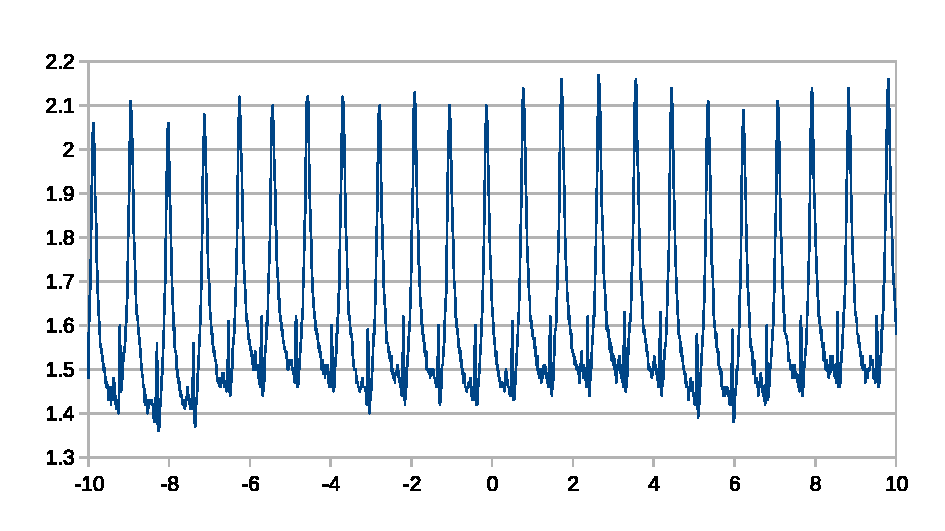
\includegraphics[scale=1,width=0.9\textwidth]{Images/HR69.pdf} 
		\caption{Sample Trace of ECG waveform with Heart Rate = 69}
	\end{center}
\end{figure}

\section{Synthetic Sensors}
\label{sec:SyntheticSensors}
By analyzing the two primary sensors, additional sensor data can be derived.  These derived measurements are called “synthetic sensors”. A synthetic sensor aggregates the data from other “real” sensors and calculates a measurement for a sensor type normally requiring additional hardware \cite{Fortier2009}. The synthetic sensor concept is illustrated in \cref{fig:SyntheticSensor}.

\begin{figure}
	\begin{center}
		\label{fig:SyntheticSensor}
		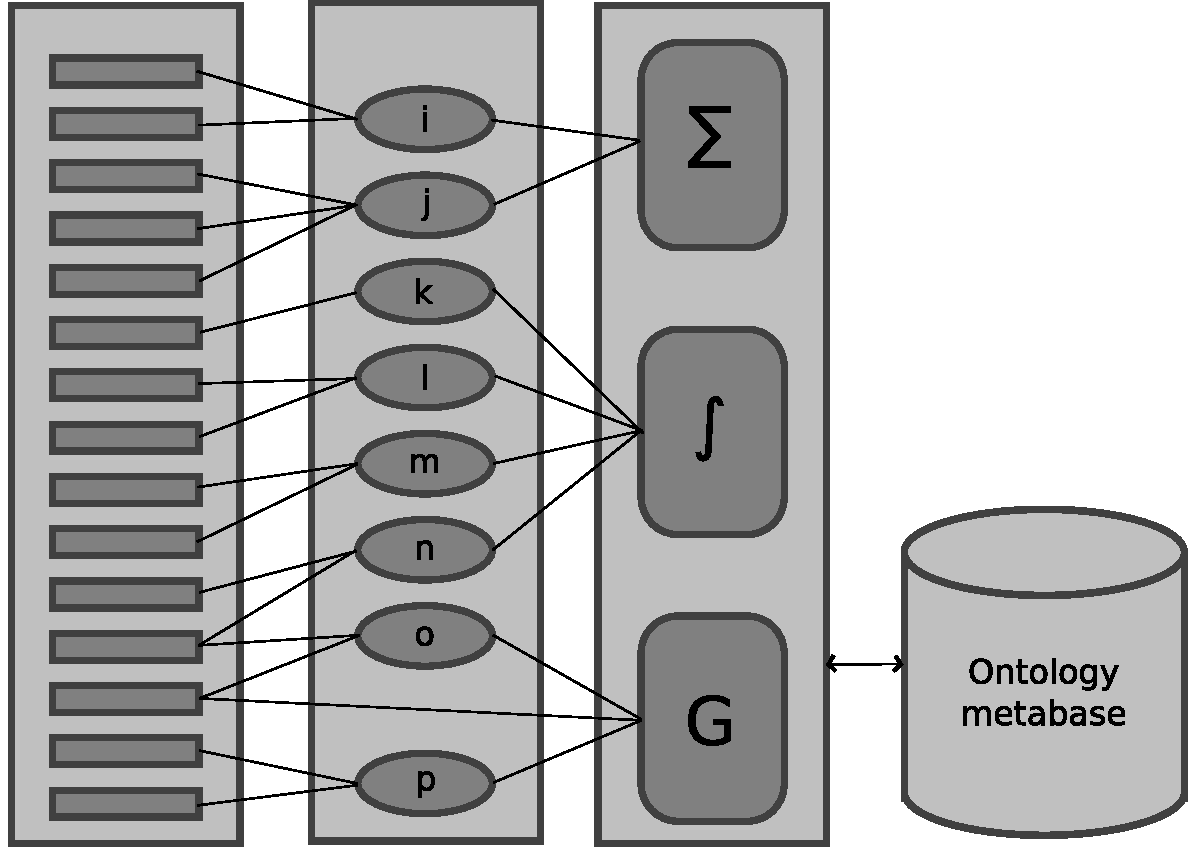
\includegraphics[scale=1,width=0.9\textwidth]{Images/syntheticSensor.pdf} 
		\caption{Synthetic Sensor Concepts for the Medical Domain}
	\end{center}
\end{figure}

\subsection{Pulse Rate}
\label{subsec:PulseRate}
The first and simplest synthetic sensor to construct, given the real transducers, is a pulse rate sensor. A combination of signal processing techniques are used to identify the QRS complex of an ECG signal, to derive the pulse rate  \cite{Chaitanya2011}. The number of QRS complexes per minute is the derived measurement of pulse rate, in beats per minute \cite{Scully2012}. Examining \cref{fig:20SecondEcg} shows a twenty-second ECG trace. \cref{fig:PulseRateCalc} shows the calculations necessary to determine heart rate.
\begin{figure}
	\begin{center}
		\label{fig:PulseRateCalc}
		$\frac{23 R-waves}{20 seconds}*\frac{60 seconds}{1 minute}=69 \frac{beats}{minute}$
		\caption{Basic Pulse rate calculation}
	\end{center}
\end{figure}

However, it is also possible to calculate the pulse rate on the R-R interval as shown in \cref{fig:RR_PulseRateCalc}. Calculating the heart rate in this way can produce fluctuations and a moving average based on the R-R interval can provide a more stable result.

\begin{figure}
	\begin{center}
		\label{fig:RR_PulseRateCalc}
		$\frac{1 beat}{T_{R-R} seconds}*\frac{60 seconds}{1 minute}=\frac{beats}{minute}$
		\caption{Heart Rate calculation from R-R interval}
	\end{center}
\end{figure}

The heart rate of a patient can be a primary indicator of heart health. If a patient's heart rate is elevated it can be an indication of tachycardia, barring other factors discussed in \nameref{sec:DataFusion}. The heart rate is a principal input into the wellness metric calculation.

\subsection{Blood pressure}
\label{subsec:BloodPressure}
\begin{figure}
	\begin{center}
		\label{fig:BP_cuff}
		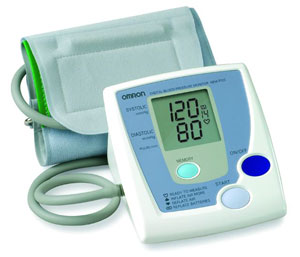
\includegraphics[scale=1,width=0.9\textwidth]{Images/BPCuff.png} 
		\caption{Commercially available blood pressure meter with auto-inflating cuff}
	\end{center}
\end{figure}

Blood pressure (BP) is a measure of the pressure exerted on the walls of the blood vessels, divided into systolic and diastolic pressures. BP is normally measured using an inflatable cuff (\cref{fig:BP_cuff}). The highest pressure occurs when blood travels through the arterial circulation by the contraction of the heart,  known as the 'systolic' blood pressure (SBP), while the 'diastolic' blood pressure (DBP) measurement is taken when the heart relaxes between beats and the pressure in the arterial circulation falls to its lowest level \cite{NOORDIN2009}. 

\begin{figure}
	\begin{center}
		\label{fig:PTT_calc}
		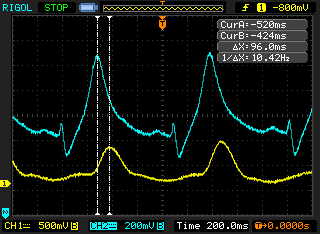
\includegraphics[scale=1,width=0.9\textwidth]{Images/PTT_Calculation.png} 
		\caption{Example calculation of Pulse Transit Time $ \Delta X $(PTT)}
	\end{center}
\end{figure}

Modern techniques for blood pressure calculation utilize a data fusion of the ECG waveform and the PPG to derive pulse wave velocity (PWV), inversely proportional to Pulse Transit time (PTT), to derive BP without the need for an inflatable cuff.  PTT is defined as the time between the detection of the pulse pressure wave in two locations on the body, usually the heart and the finger. Peak detection on the ECG and PPG trace result in two detection points (\cref{fig:PTT_calc}). Subtraction yields the PTT. Pulse transit times for the two heartbeats,shown in \cref{fig:PTT_calc}, are 1.82-1.72=0.10 seconds and 2.76-2.64=0.12 seconds. Using such a synthetic sensor has several advantages, most notably a reduced impact on the user and no moving parts. Additionally, taking BP readings with a cuff can only be performed intermittently \cite{DeMey1995}. New non-invasive techniques allow BP to be recorded for each heartbeat allowing for continuous BP monitoring \cite{Gesche2012}. 

Calculating mean BP requires a per user calibration. During the patient's hospitalization, their blood pressure will be monitored. Each time a BP reading is taken the PTT will also be recorded. A regression can be performed since research has shown that PTT is highly correlated to BP \cite{Chan2001}. Once discharged, the calculated regression will be stored in the patient's WHIPPED system. The patient's BP can now be estimated for each heart beat.  

Further research has shown how to calculate SBP and DBP from a calibration measurement \cite{Poon2005}. A single measurement of a patient's PTT and a corresponding measurement of the patient's SBP and DBP are collected under clinicians care. Further BP readings can be collected every time a PTT is calculated using the formulas shown in \cref{fig:BPCalc}.\cite{Poon2005} Poon's method simplifies the application of the WHIPPED system.

\begin{figure}
	\begin{center}

		\label{fig:BPCalc}
		
		$DBP=\frac{1}{3}*SBP_{0} + \frac{2}{3}DBP_{0} + A*ln(\frac{PTT_{w_{0}}}{PTT_{w}})l-\frac{SBP_{0} - DBP_{0}}{3}*\frac{{PTT_{w_{0}}}^{2}}{{PTT_{w}}^{2}}$
		
		$SBP=DBP+(SBP_{0}-DBP_{0})*\frac{{PTT_{w_{0}}}^2}{{PTT_{w}}^2}$
		\caption{Blood pressure calculations, given pulse transit time }
	\end{center}
\end{figure}

For the dissertation's research, a cuff-less measurement algorithm was chosen, since it more closely matches the SWaP-C system goals. Using a PTT method to eliminate the need for additional physical sensors while still achieving acceptable results allows monitoring BP for every heartbeat without disrupting blood flow. Monitoring BP is important for patient health since high BP can cause harm to the body's blood vessels.

\subsection{Respiration Rate}
\label{subsec:RespirationRate}

Respiration is the number of breaths you take per minute. Traditional techniques in a hospital environment attached a strap across a patient's chest and based on the amount the strap was stretched the respiration rate could be calculated as the number of stretches per minute. Finding a way to derive the respiration rate with the need to attach a chest strap to a patient is necessary, since a chest strap is undesirable for the same reason an inflatable cuff is undesirable (SWaP-C). Modern hospital devices can derive the respiration rate from an ECG or PPG trace. Numerous methods have been documented such as the R-S Amplitude modulation method \cite{Dziuda2011,Noor2011} and the baseline wander method \cite{Scully2012,Ponomarenko2005} to derive the respiration signal from the ECG. A simpler band pass filter on the PPG waveform has also been used \cite{Scalise2011}. Scalise's approach has been augmented by adjusting the band pass filter based on the calculated heart rate \cite{Mason2002}.

Our literature review demonstrates that additional hardware is not needed to measure the respiration waveform of a patient. It is important to monitor respiration for CHF patients, especially in conjunction with Oxygen saturation. We seek to identify such events as apneas, and hyperventilation, and, using accelerometer data, aid in determining patient motion.
